

\tikzset{every picture/.style={line width=0.75pt}} %set default line width to 0.75pt

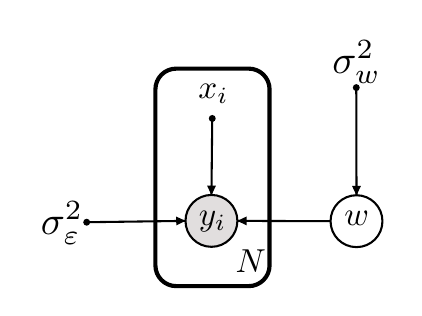
\begin{tikzpicture}[x=0.75pt,y=0.75pt,yscale=-0.5,xscale=0.5]
%uncomment if require: \path (0,300); %set diagram left start at 0, and has height of 300

\draw    (471.78, 188.29) circle [x radius= 25, y radius= 25]  ;
\draw  [fill={rgb, 255:red, 225; green, 222; blue, 222 }  ,fill opacity=1 ]  (332, 188) circle [x radius= 25, y radius= 25]  ;
\draw    (446.78,188.29) -- (357,188) ;
\draw [shift={(357,188)}, rotate = 360.18] [fill={rgb, 255:red, 0; green, 0; blue, 0 }  ] [draw opacity=0] (8.93,-4.29) -- (0,0) -- (8.93,4.29) -- (8.93,-4.29)    ;

\draw  [line width=1.5]  [rounded corners= 7.5] (278, 41.29) rectangle (388, 250.86)   ;
\draw    (211.78,189.29) -- (307,188) ;
\draw [shift={(307,188)}, rotate = 539.23] [fill={rgb, 255:red, 0; green, 0; blue, 0 }  ] [draw opacity=0] (8.93,-4.29) -- (0,0) -- (8.93,4.29) -- (8.93,-4.29)    ;
\draw [shift={(211.78,189.29)}, rotate = 359.23] [fill={rgb, 255:red, 0; green, 0; blue, 0 }  ] [draw opacity=0]    (0, 0) circle [x radius= 3.35, y radius= 3.35]   ;
\draw    (471.56,59.57) -- (471.78,163.29) ;
\draw [shift={(471.78,163.29)}, rotate = 269.88] [fill={rgb, 255:red, 0; green, 0; blue, 0 }  ] [draw opacity=0] (8.93,-4.29) -- (0,0) -- (8.93,4.29) -- (8.93,-4.29)    ;
\draw [shift={(471.56,59.57)}, rotate = 89.88] [fill={rgb, 255:red, 0; green, 0; blue, 0 }  ] [draw opacity=0]    (0, 0) circle [x radius= 3.35, y radius= 3.35]   ;
\draw    (332.78,89.29) -- (332,163) ;
\draw [shift={(332,163)}, rotate = 270.61] [fill={rgb, 255:red, 0; green, 0; blue, 0 }  ] [draw opacity=0] (8.93,-4.29) -- (0,0) -- (8.93,4.29) -- (8.93,-4.29)    ;
\draw [shift={(332.78,89.29)}, rotate = 90.61] [fill={rgb, 255:red, 0; green, 0; blue, 0 }  ] [draw opacity=0]    (0, 0) circle [x radius= 3.35, y radius= 3.35]   ;


\draw (472,186) node [scale=1.2]  {$\boldsymbol{w}$};
\draw (333,189) node [scale=1.2]  {$y_{i}$};
\draw (370,227) node [scale=1.2]  {$N$};
\draw (188,190) node [scale=1.44]  {$\sigma ^{2}_{\varepsilon }$};
\draw (472,35) node [scale=1.44]  {$\sigma ^{2}_{w}$};
\draw (334,66) node [scale=1.2]  {$x_{i}$};


\end{tikzpicture}
